\documentclass[10pt,a4paper]{article}
\usepackage{amsmath,amssymb,bm,makeidx,subfigure}
\usepackage[italian,english]{babel}
\usepackage[center,small]{caption}[2007/01/07]
\usepackage{fancyhdr}
\usepackage{color}
\usepackage{graphicx}

\definecolor{blu}{rgb}{0,0,1}
\definecolor{verde}{rgb}{0,1,0}
\definecolor{rosso}{rgb}{1,0,0}
\definecolor{viola}{rgb}{1,0,1}
\definecolor{arancio}{rgb}{1,0.5,0}
\definecolor{celeste}{rgb}{0,1,1}
\definecolor{rosa}{rgb}{1,0.3,0.5}

\oddsidemargin = 12pt
\topmargin = 0pt
\textwidth = 440pt
\textheight = 650pt

\makeindex

\begin{document}

\section{Expansion of the Sudakov form factor}

In this section I work out the expansion of the quark Sudakov form
factor to $\mathcal{O}(\alpha_s^2)$. The Sudakov form factor is
independent of the process and thus the same expansion can be used for
example for Drell-Yan and SIDIS.\footnote{Note that for
  gluon-initiated processes the expression will be different.} One
crucial point is that the expansion will be done in the so-called
$\zeta$-prescription introduced in Ref.~\cite{Scimemi:2017etj}.

The Sudakov form factor we are considering here is essentially the
square of the quark evolution factor deriving from the solution of the
Collins-Soper (CS) equations. As is well known, the CS equations
govern the evolution of TMD distributions in two independent
factorisation scales $\mu$ and $\zeta$. Usually, $\mu$ and $\zeta$ are
related to each other by assuming that $\mu=\sqrt{\zeta}$. This
particular choice reduces the degrees of freedom of the problem. On
the other hand, as observed in Ref.~\cite{Scimemi:2017etj}, this
choice does not help cure large logarithms that appear in the matching
functions. The mutual independence of $\mu$ and $\zeta$ can be
exploited to guarantee that such large logarithms are reabsorbed in
the definition of the scale $\zeta$ as a function of $\mu$ (or
viceversa). This is the basic observation at the base of the
$\zeta$-prescription that achieves this goal by assuming
$\zeta\equiv\zeta(\mu)$ and requiring that the total derivative of TMD
distribution $F$ with respect to $\mu$ is zero:
\begin{equation}\label{eq:zetapresc}
\mu^2\frac{dF\left(x,b;\mu,\zeta(\mu)\right)}{d\mu^2} = 0.
\end{equation}
This naturally leads to a differential equation in $\zeta(\mu)$
involving the CS anomalous dimensions and $\Gamma_{\rm cusp}$ that can
be solved order by order in $\alpha_s$. The exact form of the function
$\zeta(\mu)$ has to be taken into account when expanding the Sudakov
form factor.

The exact form of the Sudakov form factor, that we remind to be the
squared evolution factor deriving from the solution of the CS
equations and the evolves a pair of quark TMD distributions in $b$
space from the scales $(\mu_i,\zeta_i)$ to $(\mu_f,\zeta_f)$, is:
\begin{equation}\label{eq:sudakov}
\left[R(\mu_i,\zeta_i\rightarrow
  \mu_f,\zeta_f;b)\right]^2=\exp\left[\int_{\mu_i^2}^{\mu_f^2}\frac{d\mu^2}{\mu^2}\left(-\gamma_V+\Gamma_{\rm
    cusp}\ln\left(\frac{\mu^2}{\zeta_f}\right)\right)-2\mathcal{D}\ln\left(\frac{\zeta_f}{\zeta_i}\right)\right].
\end{equation}
where the following perturbative expansion hold:
\begin{equation}
\gamma_V = \sum_{n=1}a_s^n
\gamma_V^{(n)}\,\quad \Gamma_{\rm cusp} =
\sum_{n=1}a_s^n \Gamma_{\rm cusp}^{(n)}\,,
\end{equation}
and:
\begin{equation}
\mathcal{D} =
\sum_{n=1}a_s^{n}\sum_{k=0}^n d^{(n,k)}L^k\,,
\end{equation}
where I have defined:
\begin{equation}\label{eq:definitions}
  a_s(\mu) = \frac{\alpha_s(\mu)}{4\pi}\quad\mbox{and}\quad L\equiv \ln\left(\frac{b^2\mu_i^2}{4e^{-2\gamma_E}}\right)\,.
\end{equation}
The perturbative coefficients, $\gamma_V^{(n)}$,
$\Gamma_{\rm cusp}^{(n)}$, and $d^{(n,k)}$ are know up to the order
necessary to implement NNLL evolution.\footnote{In fact, with the only
  exception of $\Gamma_{\rm cusp}^{(4)}$, it would be possible to
  implement evolution up to N$^3$LL.} The final scales $\mu_f$ and
$\zeta_f$ are usually taken to be equal to
$\mu_f=\sqrt{\zeta}=\kappa Q$, where $Q$ is, for example the
virtuality of the exchanged photon in DIS and the invariant mass of
the lepton pair in Drell-Yan. In addition, using the
$\zeta$-prescription, we set:
\begin{equation}
\zeta_i \equiv \zeta(\mu_i) = \mu_i^2
\exp\left(\sum_{n=0}a_s^n\sum_{k=0}^{n+1}\ell^{(n,k)}L^k\right)
\end{equation}
where the coefficients $\ell^{(n,k)}$ are constants.

Before expanding the exponential we need to write its argument as a
polynomial in $\alpha_s$ (or better $a_s$) computed in $Q$. These
terms will in turn multiply powers of $\ln(Q)$. In view of the
integral over the impact parameter $b$ needed to obtain cross sections
differential in the transverse momentum $q_T$, we need to assign
$\mu_i$ a dependence on $b$. Despite this dependence is arbitrary and
needs only be dimensionally correct , the most natural choice is:
\begin{equation}
  \mu_i=\frac{C_0}{b}\,,\quad\mbox{with}\quad C_0=2e^{-\gamma_E}\,.
\end{equation}
This choice is such that $L$ defined in Eq.~(\ref{eq:definitions})
vanishes so that:
\begin{equation}
  \mathcal{D} =
  \sum_{n=1}a_s^{n}d^{(n,0)}
\end{equation}
and:
\begin{equation}
\zeta(\mu_i) =\frac{C_0^2}{b^2}
\exp\left(\sum_{n=0}a_s^n\ell^{(n,0)}\right)\,.
\end{equation}

This way the Sudakov form factor in Eq.~(\ref{eq:sudakov}) reads:
\begin{equation}\label{eq:expexp}
\begin{array}{rcl}
  \displaystyle \left[R(Q,b)\right]^2&=&\displaystyle \exp\bigg\{-\sum_{n=1}^2\int_{C_0^2/b^2}^{Q^2}\frac{d\mu^2}{\mu^2}a_s^n(\mu)\left[\gamma_V^{(n)}+\Gamma_{\rm
                                         cusp}^{(n)}\ln\left(\frac{Q^2}{\mu^2}\right)\right]\\
  \\
                                     &+&\displaystyle  2
                                         \sum_{n=1}^2a_s^{n}\left(\frac{C_0}{b}\right)d^{(n,0)}\left[-\ln\left(\frac{b^2Q^2}{C_0^2}\right)+\ell^{(0,0)}+a_s\left(\frac{C_0}{b}\right)\ell^{(1,0)}\right]\bigg\}\,,
\end{array}
\end{equation}
where we limited the contributions in the exponential to
$\mathcal{O}(a_s^2)$ that is the order we need. Now, using the RGE:
\begin{equation}
\mu^2\frac{da_s}{d\mu^2}=-\beta_0a_s^2(\mu)\,,
\end{equation}
whose solution is:
\begin{equation}
a_s(\mu) = \frac{a_s(Q)}{1-a_s(Q)\beta_0\ln(\mu^2/Q^2)}\simeq a_s(Q)\left[1+a_s(Q)\beta_0\ln(Q^2/\mu^2)+\mathcal{O}(a_s^2)\right]\,,
\end{equation}
we write every instance of $a_s$ appearing in Eq.~(\ref{eq:expexp}) in
terms of $a_s(Q)$ and finally retain only terms up to $a_s^2(Q)$:
\begin{equation}\label{eq:sudint}
\begin{array}{rcl}
  \displaystyle \left[R(Q,b)\right]^2&=&\displaystyle \exp\bigg\{-a_s(Q)\int_{C_0^2/b^2}^{Q^2}\frac{d\mu^2}{\mu^2}\left[\gamma_V^{(1)}+\Gamma_{\rm
                                         cusp}^{(1)}\ln\left(\frac{Q^2}{\mu^2}\right)\right]\\
  \\
  &-&\displaystyle a_s^2(Q) \int_{C_0^2/b^2}^{Q^2}\frac{d\mu^2}{\mu^2}\left[\gamma_V^{(2)}+\left(\Gamma_{\rm
                                         cusp}^{(2)}+\gamma_V^{(1)}\beta_0 \right)\ln\left(\frac{Q^2}{\mu^2}\right)+\Gamma_{\rm
                                         cusp}^{(1)}\beta_0\ln^2\left(\frac{Q^2}{\mu^2}\right)\right]\\
  \\
                                     &+&\displaystyle  2
                                         a_s(Q) \left[d^{(1,0)}\ell^{(0,0)}-d^{(1,0)}\ln\left(\frac{b^2Q^2}{C_0^2}\right)\right]\\
  \\ &+&\displaystyle  2 a_s^{2}(Q) \left[d^{(2,0)}\ell^{(0,0)} +
         d^{(1,0)}\ell^{(1,0)}+\left(-d^{(2,0)}+d^{(1,0)}\beta_0
         \ell^{(0,0)}\right)\ln\left(\frac{b^2Q^2}{C_0^2}\right)-d^{(1,0)}\beta_0
         \ln^2\left(\frac{b^2Q^2}{C_0^2}\right) \right]\bigg\}\,.
\end{array}
\end{equation}
The final step before carrying out the expansion is that of resolving
the integrals:
\begin{equation}
\int_{C_0^2/b^2}^{Q^2}\frac{d\mu^2}{\mu^2}\ln^k\left(\frac{Q^2}{\mu^2}\right)
= \int_{\ln(C_0^2/b^2)}^{\ln
  Q^2}d\ln\mu^2\ln^k\left(\frac{Q^2}{\mu^2}\right) = \int^{\ln(b^2Q^2/C_0^2)}_{0}dx\,x^k=\frac{1}{k+1}\ln^{k+1}\left(\frac{b^2Q^2}{C_0^2}\right)\,.
\end{equation}
If I define:
\begin{equation}
\mathcal{L}\equiv \ln\left(\frac{b^2Q^2}{C_0^2}\right)\,,
\end{equation}
the Sudakov form fact in Eq.~\ref{eq:sudint} reads:
\begin{equation}
\begin{array}{rcl}
  \displaystyle \left[R(Q,\mathcal{L})\right]^2&=&\displaystyle \exp\bigg\{a_s(Q)\left[2d^{(1,0)}\ell^{(0,0)}-\left(\gamma_V^{(1)}+2d^{(1,0)}\right)\mathcal{L}-\frac{1}{2}\Gamma_{\rm
                                         cusp}^{(1)}\mathcal{L}^2\right]\\
  \\
                                     &+&\displaystyle a_s^2(Q) \bigg[2d^{(2,0)}\ell^{(0,0)} +
                                         2d^{(1,0)}\ell^{(1,0)}+\left(-2d^{(2,0)}+2d^{(1,0)}\beta_0
                                         \ell^{(0,0)}-\gamma_V^{(2)}\right)\mathcal{L}\\
  \\
                                     &-&\displaystyle \frac12\left(4d^{(1,0)}\beta_0+\Gamma_{\rm
                                         cusp}^{(2)}+\gamma_V^{(1)}\beta_0 \right) \mathcal{L}^2-\frac13\Gamma_{\rm
                                         cusp}^{(1)}\beta_0 \mathcal{L}^3\bigg]\bigg\}\,,
\end{array}
\end{equation}
that can be conveniently written as:
\begin{equation}\label{eq:SudCompact}
  \displaystyle \left[R(Q,\mathcal{L})\right]^2=\exp\left\{\sum_{n=1}^2a_s^n(Q)\sum_{k=0}^{n+1}S^{(n,k)}\mathcal{L}^k\right\}\,,
\end{equation}
with:
\begin{equation}
\begin{array}{l}
\displaystyle S^{(1,0)} =
  2d^{(1,0)}\ell^{(0,0)}=0\,,\quad\displaystyle S^{(1,1)} =
  -\left(\gamma_V^{(1)}+2d^{(1,0)}\right)=6 C_F\,,\quad\displaystyle
                                                   S^{(1,2)} =
  -\frac{1}{2}\Gamma_{\rm cusp}^{(1)}= -2C_F\,,\\
\\
\displaystyle S^{(2,0)} = 2d^{(2,0)}\ell^{(0,0)} +
  2d^{(1,0)}\ell^{(1,0)}\,,\quad\displaystyle S^{(2,1)} =
                           \left(-2d^{(2,0)}+2d^{(1,0)}\beta_0
  \ell^{(0,0)}-\gamma_V^{(2)}\right)\,,\\
\\
\displaystyle S^{(2,2)} = -\frac12\left(4d^{(1,0)}\beta_0+\Gamma_{\rm cusp}^{(2)}+\gamma_V^{(1)}\beta_0 \right)\,,\quad\displaystyle S^{(2,3)} = -\frac13\Gamma_{\rm cusp}^{(1)}\beta_0\,.
\end{array}
\end{equation}
The values of the coefficients of the anomalous dimensions and beta
function can be read from Appendix D of
Ref.~\cite{Echevarria:2016scs}. The coefficients of the expansion of
$\zeta(\mu)$ are instead reported in Eq.~(2.29) of
Ref.~\cite{Scimemi:2017etj}. For the $\mathcal{O}(a_s)$ coefficients I
reported the explicit values. This will help check the result against
those in the literature.

Eq.~(\ref{eq:SudCompact}) can be easily expanded as up to order
$a_s^2$ as:
\begin{equation}\label{eq:exp1}
\begin{array}{rcl}
  \displaystyle \left[R(Q,\mathcal{L})\right]^2&=&\displaystyle
                                         1+a_s(Q)\sum_{k=0}^{2}S^{(1,k)}\mathcal{L}^k+a_s^2(Q)\left[\sum_{k=0}^{3}S^{(2,k)}\mathcal{L}^k+\frac12\left(\sum_{k=0}^{2}S^{(1,k)}\mathcal{L}^k\right)^2\right]+\mathcal{O}(a_s^3)\\
  \\
                                     &=&\displaystyle
                                         1+a_s(Q)\sum_{k=0}^{2}S^{(1,k)}\mathcal{L}^k+a_s^2(Q)
                                         \sum_{k=0}^{4}\widetilde{S}^{(2,k)}\mathcal{L}^k
                                         +\mathcal{O}(a_s^3)\\
\\
&\equiv&\displaystyle  1+a_s(Q)R^{(1)}+a_s^2(Q)
                                         R^{(2)}+\mathcal{O}(a_s^3)\,,
\end{array}
\end{equation}
with:
\begin{equation}
\begin{array}{l}
\displaystyle  \widetilde{S}^{(2,0)}={S}^{(2,0)}+\frac12
  \left[S^{(1,0)}\right]^2\,,\\
  \\
\displaystyle    \widetilde{S}^{(2,1)}={S}^{(2,1)}+{S}^{(1,0)}{S}^{(1,1)}\\
\\
\displaystyle    \widetilde{S}^{(2,2)}={S}^{(2,2)}+\frac12 \left[S^{(1,1)}\right]^2+{S}^{(1,2)}{S}^{(1,0)}\,,\\
\\
\displaystyle   \widetilde{S}^{(2,3)}={S}^{(2,3)}+{S}^{(1,1)}{S}^{(1,2)}\\
\\
\displaystyle    \widetilde{S}^{(2,4)}=\frac12 \left[S^{(1,2)}\right]^2\,.
\end{array}
\end{equation}

Now that the expansion of the Sudakov form factor is done to
$\mathcal{O}(a_s^2)$, it can be combined to the rest of the
perturbative quantities entering the computation of the cross
section. In the following, we will concentrate on SIDIS that involves
both TMD PDFs $F$ and TMD FFs $D$. Specifically, in $b$ space the
SIDIS cross section is a combination of terms having the following
structure:
\begin{equation}
\begin{array}{rcl}
  \displaystyle B_{ij} &=& \displaystyle
                           H(Q)\,F_i(x,b;Q)\,D_j(z,b;Q)
                           =H(Q)\,\left[R(Q,\mathcal{L})\right]^2
                           \,F_i\left(x,b;\frac{C_0}{b}\right)\,D_j\left(z,b;\frac{C_0}{b}\right)\\
\\
&=& \displaystyle H(Q)\,\left[R(Q,\mathcal{L})\right]^2
                           \left[\sum_{k}
    \mathcal{C}_{ik}(x,\mathcal{L}) \mathop{\otimes}_x
    f_k\left(x;Q\right)\right]\left[\sum_{l}
    \mathbb{C}_{jl}(z,\mathcal{L}) \mathop{\otimes}_z
    d_l\left(z;Q\right)\right]\\
\\
&\equiv& \displaystyle \sum_{kl}\hat{B}_{ij,kl}(x,z;b)\mathop{\otimes}_{x}f_k \mathop{\otimes}_{z}d_l \,,
\end{array}
\end{equation}
where $f_k$ and $d_l$ are the (non-perturbative) collinear PDFs and FFs,
respectively. The other terms, including $R^2$, are perturbatively
computable as:
\begin{equation}
\begin{array}{l}
\displaystyle H(Q) = 1+a_s(Q)H^{(1)}+a_s^2(Q)H^{(2)}+\mathcal{O}(a_s^3)\,,\\
\\
\displaystyle \mathcal{C}_{ik}(x,\mathcal{L}) = \delta_{ik}\delta(1-x)+a_s(Q)
  \mathcal{C}_{ik}^{(1)}(x,\mathcal{L}) +a_s^2(Q) \mathcal{C}_{ik}^{(2)}(x,\mathcal{L})
  +\mathcal{O}(a_s^3) \,,\\
\\
\displaystyle \mathbb{C}_{jl}(z,\mathcal{L}) = \delta_{jl}\delta(1-z)+a_s(Q) \mathbb{C}_{jl}^{(1)}(z,\mathcal{L}) +a_s^2(Q) \mathbb{C}_{jl}^{(2)}(z,\mathcal{L}) +\mathcal{O}(a_s^3) \,.
\end{array}
\end{equation}
I now need to put everything together and truncate to order $a_s^2$ in
such a way that:
\begin{equation}
\hat{B}_{ij,kl}(x,z;b) = \hat{B}_{ij,kl}^{(0)}(x,z;b)+a_s(Q) \hat{B}_{ij,kl}^{(1)}(x,z;b)+a_s^2(Q) \hat{B}_{ij,kl}^{(2)}(x,z;b)+\mathcal{O}(a_s^3) \,,
\end{equation}
with:
\begin{equation}\label{eq:pertcoefb}
\begin{array}{rcl}
  \displaystyle \hat{B}_{ij,kl}^{(0)} &=&\displaystyle
                                          \delta_{ik}\delta_{jl}\delta(1-x)\delta(1-z)\,,\\
  \\
  \displaystyle \hat{B}_{ij,kl}^{(1)} &=&\displaystyle
                                          (H^{(1)}+R^{(1)})\delta_{ik}\delta_{jl}\delta(1-x)\delta(1-z)\\
  \\
                                      &+& \mathcal{C}_{ik}^{(1)}(x,\mathcal{L})\delta_{jl}\delta(1-z) + \delta_{ik}\delta(1-x)\mathbb{C}_{jl}^{(1)}(z,\mathcal{L})\\
  \\
  \displaystyle \hat{B}_{ij,kl}^{(2)} &=& \displaystyle
                                          (H^{(2)}+H^{(1)}R^{(1)}+R^{(2)})
                                          \delta_{ik}\delta_{jl}\delta(1-x)\delta(1-z)\\
  \\
                                      &+&\displaystyle
                                          (H^{(1)}+R^{(1)})\left[\mathcal{C}_{ik}^{(1)}(x,\mathcal{L})\delta_{jl}\delta(1-z)
                                          +
                                          \delta_{ik}\delta(1-x)\mathbb{C}_{jl}^{(1)}(z,\mathcal{L})\right]\\
  \\
                                      &+& \mathcal{C}_{ik}^{(2)}(x,\mathcal{L})\delta_{jl}\delta(1-z) + 
                                          \mathcal{C}_{ik}^{(1)}(x,\mathcal{L})\mathbb{C}_{jl}^{(1)}(z,\mathcal{L})
                                          +\delta_{ik}\delta(1-x)\mathbb{C}_{jl}^{(2)}(z,\mathcal{L})
\end{array}
\end{equation}

Despite we derived the expansion of the resummed cross section up to
$\mathcal{O}(a_s^2)$, these are not yet the final formulas. The reason
is that, in order some of the terms of the expansion above do not
depend on the impact parameter $b$. This means that these terms, upon
Fourier transform needed to obtain the expression in the transverse
moment $q_T$, will give rise to terms proportional to
$\delta(q_T)$. In view of the matching procedure, since the
fixed-order expression we are going to match to does not include any
$\delta(q_T)$ terms, we need to make sure that they are not
subtracted.Therefore, we need to identify and remove any term that
does not depend on $b$. In fact, by construction, this is equivalent
to leave only terms proportional to a power of $\mathcal{L}$. In order
to do so, we start observing that the hard factor $H$ does not contain
any $\mathcal{L}$. In addition, we have to pay attention to the
coefficients $R^{(n)}$ because they are polynomials in $\mathcal{L}$
but also include a constant term ($\mathcal{L}^0$). Finally, the
$\zeta$-prescription, Eq.~(\ref{eq:zetapresc}), provides us with a
simple recipe to compute the logarithmic terms of the matching
functions $\mathcal{C}_{ik}^{(n)}$ and
$\mathbb{C}_{jl}^{(n)}$. Specifically, the condition of independence
of the TMD PDFs and FFs from the factorisation scale $\mu$ is such
that TMDs behave like physical observable (\textit{e.g.}
deep-inelastic-scattering or single-inclusive-annihilation structure
functions) and thus obey the standard scale variation rules derived,
for example, in Eq.~(2.17) of Ref.~\cite{vanNeerven:2000uj}. More in
particular, one finds that the matching function coefficients s have
the usual logarithmic structure:
\begin{equation}
\mathcal{C}_{ij}^{(n)}(x,\mathcal{L}) =
\sum_{k=0}^{n}\mathcal{C}_{ij}^{(n,k)}(x)\mathcal{L}^k\quad\mbox{and}\quad \mathbb{C}_{ij}^{(n)}(x,\mathcal{L}) = \sum_{k=0}^{n}\mathbb{C}_{ij}^{(n,k)}(x)\mathcal{L}^k \,,
\end{equation}
where the non-logarithmic terms $\mathcal{C}_{ij}^{(n,0)}$ and
$\mathbb{C}_{ij}^{(n,0)}$ have to be computed explicitly while the
other terms proportional to a positive power of $\mathcal{L}$ can be
expressed in terms of the non-logarithmic term of the previous orders
and of the coefficients of the DGLAP splitting functions and of the
QCD $\beta$ function:
\begin{equation}
\begin{array}{rcl}
  \mathcal{C}_{ij}^{(1,1)}(x) &=& -\mathcal{P}_{ij}^{(1)}(x) \,,\\
  \\
  \mathcal{C}_{ij}^{(2,1)}(x) &=& -\left(\mathcal{P}_{ij}^{(2)}(x)+\mathcal{C}_{ik}^{(1,0)}(x)
                                  \otimes
                                  \mathcal{P}_{kj}^{(1)}(x)-\beta_0
                                  \mathcal{C}_{ij}^{(1,0)}(x) \right)\,,\\
  \\
  \mathcal{C}_{ij}^{(2,2)}(x) &=&\displaystyle
                                  \frac12\left(\mathcal{P}_{ik}^{(1)}(x)\otimes \mathcal{P}_{kj}^{(1)}(x)-\beta_0 \mathcal{P}_{ij}^{(1)}(x)\right)\,,\\
\end{array}
\end{equation}
and:
\begin{equation}
\begin{array}{rcl}
  \mathbb{C}_{ij}^{(1,1)}(x) &=& -\mathbb{P}_{ij}^{(1)}(x) \,,\\
  \\
  \mathbb{C}_{ij}^{(2,1)}(x) &=& -\left(\mathbb{P}_{ij}^{(2)}(x)+\mathbb{C}_{ik}^{(1,0)}(x)
                                  \otimes
                                  \mathbb{P}_{kj}^{(1)}(x)-\beta_0
                                  \mathbb{C}_{ij}^{(1,0)}(x) \right)\,,\\
  \\
  \mathbb{C}_{ij}^{(2,2)}(x) &=&\displaystyle
                                  \frac12\left(\mathbb{P}_{ik}^{(1)}(x)\otimes \mathbb{P}_{kj}^{(1)}(x)-\beta_0 \mathbb{P}_{ij}^{(1)}(x)\right)\,,\\
\end{array}
\end{equation}
where $\mathcal{P}_{ij}^{(n)}$ and $\mathbb{P}_{ij}^{(n)}$ are the
coefficients of the $a_s^n$ terms of the space- and time-like
splitting functions, respectively. With this information at hand,
knowing the logarithmic expansion of the coefficients $R^{(n)}$, and
keeping in mind that the hard coefficients $H^{(n)}$ do not contain
any logarithms, we can organize the coefficients
inEq.~(\ref{eq:pertcoefb}) in terms of powers of
$\mathcal{L}$. Specifically, we find that:
\begin{equation}
\hat{B}_{ij,kl}^{(n)} = \sum_{p=0}^{2n}\hat{B}_{ij,kl}^{(n,p)}\mathcal{L}^p\,,
\end{equation}
with the $\mathcal{O}(1)$ coefficient being:
\begin{equation}
\begin{array}{rcl}
  \hat{B}_{ij,kl}^{(0,0)} &=& \delta_{ik}\delta_{kl}\delta(1-x)
                              \delta(1-z)\,,
\end{array}
\end{equation}
the $\mathcal{O}(a_s)$ coefficients being:
\begin{equation}
\begin{array}{rcl}
  \hat{B}_{ij,kl}^{(1,0)} &=&\displaystyle
                              (H^{(1)}+S^{(1,0)})\delta_{ik}\delta_{jl}\delta(1-x)\delta(1-z)+ \mathcal{C}_{ik}^{(1,0)}(x)\delta_{jl}\delta(1-z) + \delta_{ik}\delta(1-x)\mathbb{C}_{jl}^{(1,0)}(z)\,,\\
  \\
  \hat{B}_{ij,kl}^{(1,1)} &=& S^{(1,1)}\delta_{ik}\delta_{jl}\delta(1-x)\delta(1-z)+ \mathcal{C}_{ik}^{(1,1)}(x)\delta_{jl}\delta(1-z) + \delta_{ik}\delta(1-x)\mathbb{C}_{jl}^{(1,1)}(z) \,,\\
  \\
  \hat{B}_{ij,kl}^{(1,2)} &=&
                              S^{(1,2)}\delta_{ik}\delta_{jl}\delta(1-x)\delta(1-z)
\end{array}
\end{equation}
and the $\mathcal{O}(a_s^2)$ coefficients being:
\begin{equation}
\begin{array}{rcl}
  \hat{B}_{ij,kl}^{(2,0)} &=&\displaystyle (H^{(2)}+H^{(1)}S^{(1,0)}+\widetilde{S}^{(2,0)})
                              \delta_{ik}\delta_{jl}\delta(1-x)\delta(1-z) \,,\\
  \\
                          &+&\displaystyle
                              (H^{(1)}+S^{(1,0)})\left[\mathcal{C}_{ik}^{(1,0)}(x)\delta_{jl}\delta(1-z)
                              +
                              \delta_{ik}\delta(1-x)\mathbb{C}_{jl}^{(1,0)}(z)\right]\\
  \\
                          &+&\displaystyle \mathcal{C}_{ik}^{(2,0)}(x)\delta_{jl}\delta(1-z) + 
                              \mathcal{C}_{ik}^{(1,0)}(x)\mathbb{C}_{jl}^{(1,0)}(z)
                              +\delta_{ik}\delta(1-x)\mathbb{C}_{jl}^{(2,0)}(z)\\

  \\
  \hat{B}_{ij,kl}^{(2,1)} &=&\displaystyle (H^{(1)}S^{(1,1)}+\widetilde{S}^{(2,1)})
                              \delta_{ik}\delta_{jl}\delta(1-x)\delta(1-z)\\
  \\
                          &+& \displaystyle
                              (H^{(1)}+S^{(1,0)})\left[\mathcal{C}_{ik}^{(1,1)}(x)\delta_{jl}\delta(1-z)
                              +
                              \delta_{ik}\delta(1-x)\mathbb{C}_{jl}^{(1,1)}(z)\right]\\
  \\
                          &+&
                              S^{(1,1)}\left[\mathcal{C}_{ik}^{(1,0)}(x)\delta_{jl}\delta(1-z)
                              +
                              \delta_{ik}\delta(1-x)\mathbb{C}_{jl}^{(1,0)}(z)\right]\\
  \\
                          &+& \mathcal{C}_{ik}^{(2,1)}(x)\delta_{jl}\delta(1-z) + 
                              \mathcal{C}_{ik}^{(1,1)}(x)\mathbb{C}_{jl}^{(1,0)}(z) +\mathcal{C}_{ik}^{(1,0)}(x)\mathbb{C}_{jl}^{(1,1)}(z)
                              +\delta_{ik}\delta(1-x)\mathbb{C}_{jl}^{(2,1)}(z)\\
  \\
  \hat{B}_{ij,kl}^{(2,2)} &=&\displaystyle (H^{(1)}S^{(1,2)}+\widetilde{S}^{(2,2)})
                              \delta_{ik}\delta_{jl}\delta(1-x)\delta(1-z)\\
  \\
                          &+&\displaystyle
                              \widetilde{S}^{(1,2)}\left[\mathcal{C}_{ik}^{(1,0)}(x)\delta_{jl}\delta(1-z)+\delta_{ik}\delta(1-x)\mathbb{C}_{jl}^{(1,0)}(z)\right]\\
  \\
                          &+&\displaystyle
                              S^{(1,1)}\left[\mathcal{C}_{ik}^{(1,1)}(x)\delta_{jl}\delta(1-z)+\delta_{ik}\delta(1-x)\mathbb{C}_{jl}^{(1,1)}(z)\right]\\
  \\
                          &+& \mathcal{C}_{ik}^{(2,2)}(x)\delta_{jl}\delta(1-z) + 
                              \mathcal{C}_{ik}^{(1,1)}(x)\mathbb{C}_{jl}^{(1,1)}(z)
                              +\delta_{ik}\delta(1-x)\mathbb{C}_{jl}^{(2,2)}(z)\\
  \\
  \hat{B}_{ij,kl}^{(2,3)} &=&\displaystyle
                              \widetilde{S}^{(2,3)}\delta_{ik}\delta_{jl}\delta(1-x)\delta(1-z)
                              + S^{(1,2)}\left[\mathcal{C}_{ik}^{(1,1)}(x)\delta_{jl}\delta(1-z)
                              +
                              \delta_{ik}\delta(1-x)\mathbb{C}_{jl}^{(1,1)}(z)\right]
  \\
  \\
  \hat{B}_{ij,kl}^{(2,4)} &=&\displaystyle \widetilde{S}^{(2,4)}\delta_{ik}\delta_{jl}\delta(1-x)\delta(1-z)
\end{array}
\end{equation}

In order to obtain a differential cross section in $q_T$, we need to
take the Fourier transform of $\hat{B}_{ij,kl}$, that is:
\begin{equation}
 \hat{B}_{ij,kl}(x,z;q_T) \equiv \int\frac{d^2\mathbf{b}}{4\pi} e^{i \mathbf{b}\cdot
  \mathbf{q}_T} \hat{B}_{ij,kl}(x,z;b) = \sum_{n=0}^2a_s^n(Q)\sum_{p=0}^{2n}\hat{B}_{ij,kl}^{(n,p)}(x,z) I_p(q_T)\,,
\end{equation}
where I have defined:
\begin{equation}
I_p(q_T) = \int\frac{d^2\mathbf{b}}{4\pi} e^{i \mathbf{b}\cdot
  \mathbf{q}_T}\mathcal{L}^p=\int\frac{d^2\mathbf{b}}{4\pi} e^{i \mathbf{b}\cdot
  \mathbf{q}_T}\ln^p\left(\frac{b^2Q^2}{C_0^2}\right) = \frac12\int_0^\infty db\,b J_0(bq_T) \ln^p\left(\frac{b^2Q^2}{C_0^2}\right)\,.
\end{equation}
Results for $I_p$ have been computed up to $p=4$ in Eq.~(136) of
Appendix B of Ref.~\cite{Bozzi:2005wk}. Specifically, and including
the trivial tranform with $p=0$, they read:
\begin{equation}
\begin{array}{l}
\displaystyle I_0(q_T) = \delta(q_T)\,,\\
\\
\displaystyle I_1(q_T) = - \frac{1}{q_T^2}\,,\\
\\
\displaystyle I_2(q_T) = - \frac{2}{q_T^2}\ln\left(\frac{Q^2}{q_T^2}\right) \,,\\
\\
\displaystyle I_3(q_T) = - \frac{3}{q_T^2}\ln^2\left(\frac{Q^2}{q_T^2}\right) \,,\\
\\
\displaystyle I_4(q_T) = - \frac{4}{q_T^2}\left[\ln^3\left(\frac{Q^2}{q_T^2}\right)-4\zeta_3\right]\,.
\end{array}
\end{equation}
As clear from the transforms above, all terms with $p=0$ will be
proportional to $\delta(q_T)$. We do not need to consider these terms
because analogous terms are not included in the fixed-order
calculation and thus does not need to be subtracted. Therefore, we write:
\begin{equation}\label{eq:finalformula}
  \hat{B}_{ij,kl}(x,z;q_T) =
  \sum_{n=1}^2a_s^n(Q)\sum_{p=1}^{2n}\hat{B}_{ij,kl}^{(n,p)}(x,z)
  I_p(q_T)+ \left(\sum_{n=0}^2a_s^n(Q)\hat{B}_{ij,kl}^{(n,0)}(x,z)\right)\delta(q_T)+\mathcal{O}(a_s^3)\,,
\end{equation}
and we are not going to consider the term proportional to
$\delta(q_T)$, even though all terms have been derived above.

As clear from Eq.~(\ref{eq:finalformula}), removing all terms
proportional to $\delta(q_T)$ also means removing the full
$\mathcal{O}(1)$ terms such that leading-order term is now
$\mathcal{O}(a_s)$.

In order to validate the results above, it is opportune to compare the
$\mathcal{O}(a_s)$ expressions to those present in the literature. To
this end, we write explicitly the expression for
$\hat{B}_{ij,kl}^{(1)}$ in $q_T$ space without the $\delta(q_T)$ term:
\begin{equation}
\begin{array}{rcl}
\hat{B}_{ij,kl}^{(1)}(x,z;q_T) &=&\displaystyle 
-\hat{B}_{ij,kl}^{(1,1)}(x,z)\mathcal{L}\frac{1}{q_T^2}
  -\hat{B}_{ij,kl}^{(1,2)}(x,z)\frac{2}{q_T^2}\ln\left(\frac{Q^2}{q_T^2}\right)\\
\\
 &=&\displaystyle
     \frac{1}{q_T^2}\bigg[4C_F\left(\ln\left(\frac{Q^2}{q_T^2}\right)-\frac{3}{2}\right)\delta_{ik}\delta_{jl}\delta(1-x)\delta(1-z)\\
\\
 &+&\displaystyle \mathcal{P}_{ik}^{(1)}(x)\delta_{jl}\delta(1-z) + \delta_{ik}\delta(1-x)\mathbb{P}_{jl}^{(1)}(z)\bigg]\,,
\end{array}
\end{equation}
so that:
\begin{equation}\label{eq:asymptfromres}
\begin{array}{rcl}
B_{ij}(x,z;q_T) &=&\displaystyle a_s(Q) \sum_{kl}\hat{B}_{ij,kl}^{(1)}\mathop{\otimes}_x
  f_k(x,Q)\mathop{\otimes}_zd_l(z,Q)+\mathcal{O}(a_s^2)\\
\\
&=&\displaystyle a_s(Q) \frac{1}{q_T^2}\bigg[4C_F\left(\ln\left(\frac{Q^2}{q_T^2}\right)-\frac{3}{2}\right) f_i(x,Q)d_j(z,Q)\\
\\
 &+&\displaystyle \left(\sum_{k}\mathcal{P}_{ik}^{(1)}(x) \mathop{\otimes}_x
  f_k(x,Q)\right)d_j(z,Q) + f_i(x,Q)\left(\sum_l\mathbb{P}_{jl}^{(1)}(z) \mathop{\otimes}_zd_l(z,Q)\right) +\mathcal{O}(a_s^2)\,.
\end{array}
\end{equation}
This result, up to som pre-factor and to selecting the right flavour
combinations,\footnote{We have purposely left the flavour indices $i$
  and $j$ unspecified because they do not necessarily run over the
  quark flavours $u$, $d$, etc. In fact, it turns out to be useful to
  adopt a different basis (usual referred to as evolution basis) that
  simplifies the structure of the products between, for example,
  PDFs/FFs and splitting functions.} nicely agrees with that of,
\textit{e.g.},
Refs.~\cite{Meng:1995yn,Nadolsky:1999kb,Collins:2016hqq}.

In order to check that the matching is actually removing the double
counting terms, it is instructive to derive
Eq.~(\ref{eq:asymptfromres}) extracting the asymptote from the
fixed-order computation at $\mathcal{O}(a_s)$. We take the expressions
for the coefficient functions from Eqs.~(106)-(109) of Appendix B of
Ref.~\cite{Nadolsky:1999kb} or from Eqs.~(4.6)-(4.20) of
Ref.~\cite{Bacchetta:2008xw}.Referring to the second reference, some
simplifications apply. First, we consider cross sections with
unpolarised projectiles ($\lambda_e=0$) over unpolarised targets
($S_\perp^\mu = 0$) and integrated over the azimuthal angles $\phi_H$
and $\phi_S$. By doing so and after a simple manipulation, the cross
section simplifies greatly and can be written in terms of structure
functions as:
\begin{equation}\label{eq:xsexinsf}
  \frac{d\sigma}{dx dy dz dq_T^2} = \frac{2\pi\alpha^2}{xyQ^2}\left[Y_+ F_{UU,T}+2(1-y)F_{UU,L}\right]=\frac{2\pi\alpha^2}{xyQ^2}Y_+\left[F_{UU,2}-\frac{y^2}{Y_+}F_{UU,L}\right]\,,
\end{equation}
with:
\begin{equation}
Y_+\equiv 1+(1-y)^2\,,
\end{equation}
and where we have defined the structure function:
\begin{equation}
F_{UU,2}\equiv F_{UU,T} + F_{UU,L}\,.
\end{equation}
Notice that, as compared to Ref.~\cite{Bacchetta:2008xw}, we have
factored out from the structure functions a further factor
$1/(\pi z^2)$\footnote{Factor $z^2$ is the consequence of the fact
  that we are writing the cross section differential in $q_T^2$ that
  is the transverse momentum of the exchanged photon while in
  Ref.~\cite{Bacchetta:2008xw} the cross section is differentila in
  $p_T^2$ that is the transverse momentum of the of the outgoing
  hadrons. Since $p_T=z q_T$, the factor $z^2$ cancels.} so that they
factorize as:
\begin{equation}\label{eq:FOxsec}
\begin{array}{rcl}
  F_{UU,S}&=&\displaystyle 
  a_s\frac{x}{Q^2}\sum_{i}e_i^2\int_x^1\frac{d\bar{x}}{\bar{x}}\int_z^1\frac{d\bar{z}}{\bar{z}}\delta\left(\frac{q_T^2}{Q^2}-\frac{(1-\bar{x})(1-\bar{z})}{\bar{x}\bar{z}}\right)\bigg[\hat{B}_{qq}^{S,
    \rm FO}(\bar{x},\bar{z},q_T)f_i\left(\frac{x}{\bar{x}}\right)
              d_i\left(\frac{z}{\bar{z}}\right)\\
\\
&+&\displaystyle \hat{B}_{qg}^{S,
    \rm FO}(\bar{x},\bar{z},q_T)f_g\left(\frac{x}{\bar{x}}\right)
              d_i\left(\frac{z}{\bar{z}}\right)+ \hat{B}_{gq}^{S,
    \rm FO}(\bar{x},\bar{z},q_T)f_i\left(\frac{x}{\bar{x}}\right)
              d_g\left(\frac{z}{\bar{z}}\right)\bigg]
+\mathcal{O}(a_s^2)\,.
\end{array}
\end{equation}
with $S=2,L$ and where the sum over $i$ runs over the active quark and
antiquark flavours and $e_i$ is the electric charge of the $i$-th
flavour. The expression for the coefficient functions are:
\begin{equation}\label{eq:Bacchettaetal}
\begin{array}{l}
\displaystyle \hat{B}_{qq}^{2,\rm FO}(x,z,q_T) = 2C_F\left[(1-x)(1-z)+4xz+\frac{1+x^2z^2}{xz}\frac{Q^2}{q_T^2}\right]\,,\\
\\
\displaystyle \hat{B}_{qq}^{L,\rm FO}(x,z,q_T) = 8C_Fxz\,,\\
\\
\displaystyle \hat{B}_{qg}^{2,\rm FO}(x,z,q_T) = 2T_R\left[[x^2+(1-x)^2][z^2+(1-z)^2]\frac{1-x}{xz^2}\frac{Q^2}{q_T^2} +8x(1-x)\right]\,,\\
\\
\displaystyle \hat{B}_{qg}^{L,\rm FO}(x,z,q_T) = 16T_Rx(1-x)\,.\\
\\
\displaystyle \hat{B}_{gq}^{2,\rm FO}(x,z,q_T) = 2C_F\left[(1-x)z+4x(1-z)+\frac{1+x^2(1-z)^2}{xz}\frac{1-z}{z}\frac{Q^2}{q_T^2}\right]\,,\\
\\
\displaystyle \hat{B}_{gq}^{L,\rm FO}(x,z,q_T) = 8C_Fx(1-z)\,,
\end{array}
\end{equation}
These expressions are enough to compute the SIDIS cross section at
$\mathcal{O}(a_s)$ in the region $q_T \lesssim Q$. In order to match
Eq.~(\ref{eq:asymptfromres}) one has to take the limit $q_T\ll Q$ and
retain in the coefficient functions only the terms enhanced as
$Q^2/q_T^2$. This automatically means that $F_{UU,L}$ does not
contribute in the $q_T\leftarrow 0$ limit:
\begin{equation}
F_{UU,L}\mathop{\longrightarrow}_{q_T\ll Q} 0\,.
\end{equation}
Another crucial observation is that the $\delta$-function in
Eq.~(\ref{eq:FOxsec}) can be expanded as follows:
\begin{equation}
  \delta\left(\frac{q_T^2}{Q^2}-\frac{(1-x)(1-z)}{xz}\right)
  =\ln\left(\frac{Q^2}{q_T^2}\right)\delta(1-x) \delta(1-z) +
  \frac{x\delta(1-z)}{(1-x)_+}+ \frac{z\delta(1-x)}{(1-z)_+} +\mathcal{O}\left(\frac{q_T^2}{Q^2}\ln\left(\frac{Q^2}{q_T^2}\right)\right)\,,
\end{equation}
so that:
\begin{equation}\label{eq:FOxsecasy}
\begin{array}{rcl}
  F_{UU,2}&\displaystyle \mathop{\longrightarrow}_{q_T\ll Q}&\displaystyle 
  a_s\frac{x}{q_T^2}\sum_{i}e_i^2\int_x^1\frac{d\bar{x}}{\bar{x}}\int_z^1\frac{d\bar{z}}{\bar{z}}\bigg[\hat{B}_{qq}^{2,
    \rm asy}(\bar{x},\bar{z},q_T)f_i\left(\frac{x}{\bar{x}}\right)
              d_i\left(\frac{z}{\bar{z}}\right)\\
\\
&+&\displaystyle \hat{B}_{qg}^{2,
    \rm asy}(\bar{x},\bar{z},q_T)f_g\left(\frac{x}{\bar{x}}\right)
              d_i\left(\frac{z}{\bar{z}}\right)+ \hat{B}_{gq}^{2,
    \rm asy}(\bar{x},\bar{z},q_T)f_i\left(\frac{x}{\bar{x}}\right)
              d_g\left(\frac{z}{\bar{z}}\right)\bigg]
+\mathcal{O}(a_s^2)\,.
\end{array}
\end{equation}
with:
\begin{equation}
\begin{array}{rcl}
  \hat{B}_{qq}^{2,\rm asy}(x,z,q_T) &=& \displaystyle  2C_F\left[2
                                        \ln\left(\frac{Q^2}{q_T^2}\right)+\frac{1+x^2}{(1-x)_+}\delta(1-z) +\delta(1-x)\frac{1+z^2}{(1-z)_+} \right]\\
  \\
                                    &=&\displaystyle 2C_F\left[2\ln\left(\frac{Q^2}{q_T^2}\right) -3\right]\delta(1-x) \delta(1-z)+\mathcal{P}_{qq}^{(1)}(x)\delta(1-z)
                                        +\delta(1-x) \mathbb{P}_{qq}^{(1)}(z)\,,\\
  \\
  \hat{B}_{qg}^{2,\rm asy}(x,z,q_T) &=& \displaystyle
                                        2T_R\left[x^2+(1-x)^2\right]\delta(1-z)=\mathcal{P}_{qg}^{(1)}(x)
                                        \delta(1-z)\,,\\
\\
  \hat{B}_{gq}^{2,\rm asy}(x,z,q_T) &=& \displaystyle  \delta(1-x)2C_F\left[\frac{1+(1-z)^2}{z}\right]=\delta(1-x)\mathbb{P}_{qg}^{(1)}(z)\,.
\end{array}
\end{equation}
It is thus easy to see that we can rewrite Eq.~(\ref{eq:FOxsecasy})
as:
\begin{equation}\label{eq:FOxsecasy2}
\begin{array}{rcl}
  F_{UU,2}&\displaystyle \mathop{\longrightarrow}_{q_T\ll Q}&\displaystyle 
  a_s\frac{x}{q_T^2}\sum_{i}e_i^2 \Bigg[4C_F\left(\ln\left(\frac{Q^2}{q_T^2}\right) -\frac{3}{2}\right) f_i\left(x\right)
              d_i\left(z\right)\\
\\
&+&\displaystyle
    \left(\sum_{k=q,g}\mathcal{P}^{(1)}_{qk}(x)\otimes f_k\left(x\right) \right)
              d_i\left(z\right)+ f_i\left(x\right)
              \left(\sum_{k=q,g}\mathbb{P}^{(1)}_{qk}(z) \otimes d_k\left(z\right)\right)\Bigg]
+\mathcal{O}(a_s^2)\,.
\end{array}
\end{equation}
Eq.~(\ref{eq:FOxsecasy2}) agrees with
Eq.~(\ref{eq:asymptfromres}). This confirms that this term removes the
double-counting terms when doing the matching.

In order to provide a version of Eq.~(\ref{eq:FOxsec}) that can be
readily implemented, we need to perform one of the integrals making
use of the $\delta$-function. We integrate over $\bar{x}$ so that we
write:
\begin{equation}
\delta\left(\frac{q_T^2}{Q^2}-\frac{(1-\bar{x})(1-\bar{z})}{\bar{x}\bar{z}}\right)
= \frac{\bar{z}\bar{x}_0^2}{1-\bar{z}}\delta(\bar{x} - \bar{x}_0)\,,
\end{equation}
with:
\begin{equation}\label{eq:x0bar}
  \bar{x}_0 = \frac{1-\bar{z}}{1-\bar{z}\left(1-\frac{q_T^2}{Q^2}\right)}\,.
\end{equation}
This allows us to write:
\begin{equation}\label{eq:FOxsecFin}
\begin{array}{rcl}
  F_{UU,S}&=&\displaystyle 
  a_s\frac{x }{Q^2}\sum_{i}e_i^2\int_z^{z_{\rm max}} \frac{d\bar{z}}{1-\bar{z}}\bar{x}_0\bigg[\hat{B}_{qq}^{S,
    \rm FO}(\bar{x}_0,\bar{z},q_T)f_i\left(\frac{x}{\bar{x}_0}\right)
              d_i\left(\frac{z}{\bar{z}}\right)\\
\\
&+&\displaystyle \hat{B}_{qg}^{S,
    \rm FO}(\bar{x}_0,\bar{z},q_T)f_g\left(\frac{x}{\bar{x}_0}\right)
              d_i\left(\frac{z}{\bar{z}}\right)+ \hat{B}_{gq}^{S,
    \rm FO}(\bar{x}_0,\bar{z},q_T)f_i\left(\frac{x}{\bar{x}_0}\right)
              d_g\left(\frac{z}{\bar{z}}\right)\bigg]
+\mathcal{O}(a_s^2)\,,
\end{array}
\end{equation}
with:
\begin{equation}
z_{\rm max} = \frac{1-x}{1-x\left(1-\frac{q_T^2}{Q^2}\right)}\,.
\end{equation}

Now I would like to rewrite the cross section above in such a way that
it matches that at $\mathcal{O}(a_s)$ of
Ref.~\cite{Daleo:2004pn}. That would allow us to confidently use the
$\mathcal{O}(a_s^2)$ calculation presented right in that reference for
the matching to the resummed calculation. This is made a little tricky
by the different notation used in Ref.~\cite{Daleo:2004pn} and from
the fact that in that paper the cross section is differential in a
different set of variables. Specifically, we would like it to be
differential in $x$, $y$, $z$, and $q_T^2$ while in
Ref.~\cite{Daleo:2004pn} it is differential in $x$, $Q^2$, $\eta$, and
$p_T^2$, where the last two are the rapidity and the transverse
momentum of the outgoing hadron, respectively. Eq.~(13) of
Ref.~\cite{Daleo:2004pn}, can be translated into our notation by
noticing that:
\begin{equation}\label{eq:Daleoetal}
\frac{d\sigma}{dxdQ^2d p_T^2 d\eta} = \frac{x}{z Q^2}\sum_{i,j}\int_z^{z_{\rm
    max}} \frac{d\bar{z}}{1-\bar{z}} f_i\left(\frac{x}{\bar{x}_0}\right)d_j\left(\frac{z}{\bar{z}}\right) \frac{d\sigma_{ij}^{(1)}}{dxdQ^2d p_T^2 d\eta}+\mathcal{O}(a_s^2)
\end{equation}
where we have exploited the $\delta$-functions in Eqs.~(18)-(20) to
get rid of the integral over $z$.\footnote{Notice that the $z$
  variable of Ref.~\cite{Daleo:2004pn} does not coincide with our
  definition.}

The $\mathcal{O}(a_s)$ partonic cross sections in Eqs.~(18)-(20) of
Ref.~\cite{Daleo:2004pn}, setting $\varepsilon=0$, can be written as:
\begin{equation}
\frac{d\sigma_{ij}^{(1)}}{dxdQ^2d p_T^2 d\eta}=\frac{2\pi \alpha^2 a_s
  e_q^2\bar{x}_0}{x Q^4}Y_+ \left[ \underbrace{\left( F_{UU,M}^{ij}(\bar{x}_0,\bar{z})+\frac{3}{2}F_{UU,L}^{ij}(\bar{x}_0,\bar{z})\right)}_{F_{UU,2}^{ij}} - \frac{y^2}{Y_+}F_{UU,L}^{ij}(\bar{x}_0,\bar{z})\right]\,.
\end{equation}
One can verify that $F_{UU,2}^{qq}(\bar{x}_0,\bar{z})$,
$F_{UU,L}^{qq}(\bar{x}_0,\bar{z})$,
$F_{UU,M}^{qg}(\bar{x}_0,\bar{z})$,
$F_{UU,L}^{qg}(\bar{x}_0,\bar{z})$,
$F_{UU,M}^{gq}(\bar{x}_0,\bar{z})$, and
$F_{UU,L}^{gq}(\bar{x}_0,\bar{z})$ exactly correspond to
$\hat{B}^{2, \rm FO}_{qq}(\bar{x}_0,\bar{z},q_T)$,
$\hat{B}^{L, \rm FO}_{qq}(\bar{x}_0,\bar{z},q_T)$,
$\hat{B}^{M, \rm FO}_{qg}(\bar{x}_0,\bar{z},q_T)$,
$\hat{B}^{L, \rm FO}_{qg}(\bar{x}_0,\bar{z},q_T)$,
$\hat{B}^{M, \rm FO}_{gq}(\bar{x}_0,\bar{z},q_T)$, and
$\hat{B}^{L, \rm FO}_{gq}(\bar{x}_0,\bar{z},q_T)$ of
Eq.~(\ref{eq:Bacchettaetal}). It is crucial to notice that the
correspondence holds only if $\bar{x}_0$ defined in
Eq.~(\ref{eq:x0bar}) as a function of $\bar{z}$ is used. As an
example, taking into account the different factors (a factor 2 for
$F_{UU,M}$ and a factor 4 for $F_{UU,L}$) and using our notation for
the integration variables ($y\rightarrow \bar{z}$,
$\rho(z=0)\rightarrow \bar{x}_0$), we read off from Eq.~(18) of
Ref.~\cite{Daleo:2004pn}:
\begin{equation}
\begin{array}{rcl}
F_{UU,M}^{qq}(\bar{x}_0,\bar{z}) &=& \displaystyle 2C_F\left[\frac{(\bar{x}_0+\bar{z})^2+2(1-\bar{x}_0-\bar{z})}{(1-\bar{x}_0)(1-\bar{z})}\right]\,,\\
\\
F_{UU,L}^{qq}(\bar{x}_0,\bar{z}) &=& \displaystyle 8C_F\bar{x_0}\bar{z}\,,
\end{array}
\end{equation}
so that:
\begin{equation}
\begin{array}{rcl}
F_{UU,2}^{qq}(\bar{x}_0,\bar{z}) &=& F_{UU,M}^{qq}(\bar{x}_0,\bar{z})+\frac{3}{2}F_{UU,L}^{qq}(\bar{x}_0,\bar{z})\\
\\
 &=& \displaystyle 2
     C_F\left[\frac{(\bar{x}_0+\bar{z})^2+2(1-\bar{x}_0-\bar{z})}{(1-\bar{x}_0)(1-\bar{z})}
     + 3\bar{x_0}\bar{z}\right]\\
\\
&=& \displaystyle 2
     C_F\left[(1-\bar{x}_0)(1-\bar{z})+4\bar{x}_0\bar{z} +\frac{1+\bar{x}_0^2\bar{z}^2}{\bar{x}_0\bar{z}}\left(\frac{\bar{x}_0\bar{z}}{(1-\bar{x}_0)(1-\bar{z})}\right)\right]\,.
\end{array}
\end{equation}
Using Eq.~(\ref{eq:x0bar}), it is easy to see that the factor in round
brackets in the last line of the equation above is equal to
$Q^2/q_T^2$. Therefore, it reduces exactly to the first relation in
Eq.~(\ref{eq:Bacchettaetal}). The same holds also for the remaining
two partonic channels.

Putting all pieces together, Eq.~(\ref{eq:Daleoetal}) can be recast as:
\begin{equation}
\frac{d\sigma}{dxdQ^2d p_T^2 d\eta} = \frac{2\pi \alpha^2
  }{z x Q^4}Y_+ \left[F_{UU,2} - \frac{y^2}{Y_+}F_{UU,L}\right]\,,
\end{equation}
with:
\begin{equation}
\begin{array}{rcl}
  F_{UU,S}&=&\displaystyle 
  a_s\frac{x }{Q^2}\sum_{i}e_i^2\int_z^{z_{\rm max}}
              \frac{d\bar{z}}{1-\bar{z}}\bar{x}_0\bigg[F^{qq}_{UU,L}(\bar{x}_0,\bar{z})f_i\left(\frac{x}{\bar{x}_0}\right)
              d_i\left(\frac{z}{\bar{z}}\right)\\
\\
&+&\displaystyle F^{qg}_{UU, L}(\bar{x}_0,\bar{z})f_g\left(\frac{x}{\bar{x}_0}\right)
              d_i\left(\frac{z}{\bar{z}}\right)+ F^{gq}_{UU, L}(\bar{x}_0,\bar{z})f_i\left(\frac{x}{\bar{x}_0}\right)
              d_g\left(\frac{z}{\bar{z}}\right)\bigg]
+\mathcal{O}(a_s^2)\,.
\end{array}
\end{equation}
Therefore, the structure of the observables is exactly the same. What
is left to work out is the Jacobian to express the cross section as
differential in the same variable as in Eq.~(\ref{eq:FOxsecFin}). What
we need is to know how the variables $Q^2$, $p_T$, and $\eta$ are
related to $y$, $z$, and $q_T$. The relevant relations are:
\begin{equation}
\left\{\begin{array}{rcl}
Q^2 &=& xyS_H\\
\\
p_T^2 &=& z^2 q_T^2\\
\\
\eta &=& \displaystyle \frac{1}{2}\ln\left(\frac{y(1-x)S_H}{q_T^2}\right)
\end{array}\right.\quad\Longrightarrow\quad dQ^2dp_T^2d\eta = \frac{zQ^2}{y} dydzdq_T^2\,.
\end{equation}
where $S_H$ is the squared center-of-mass energy of the collision, so
that:
\begin{equation}
  \frac{d\sigma}{dx dy dz dq_T^2} = \frac{zQ^2}{y}\frac{d\sigma}{dxdQ^2d p_T^2
    d\eta} = \frac{2\pi\alpha^2}{xyQ^2}Y_+\left[F_{UU,2}-\frac{y^2}{Y_+}F_{UU,L}\right]\,,
\end{equation}
exactly like in Eq.~(\ref{eq:xsexinsf}). This confirms that the
computation of Ref.~\cite{Daleo:2004pn} can be matched to the resummed
calculation provided that the correct Jacobian is taken into account.

In Fig.~\ref{fig:APFELvsTIMBA}, a comparison between the
$\mathcal{O}(a_s)$ computation of Ref.~\cite{Daleo:2004pn} for the
differential cross section in Eq.~(\ref{eq:Daleoetal}), implemented in
the computer code {\tt TIMBA}, and the implementation in the {\tt
  APFEL++} framework~\cite{Bertone:2017gds} of the expressions in
Eq.~(\ref{eq:FOxsecFin}) is presented. The cross section as a function
of the hadron transverse momentum $p_T$ obtained with {\tt APFEL++} is
displayed as ratios to {\tt TIMBA} for a representative values of the
kinematic variables.
\begin{figure}[t]
  \begin{centering}
    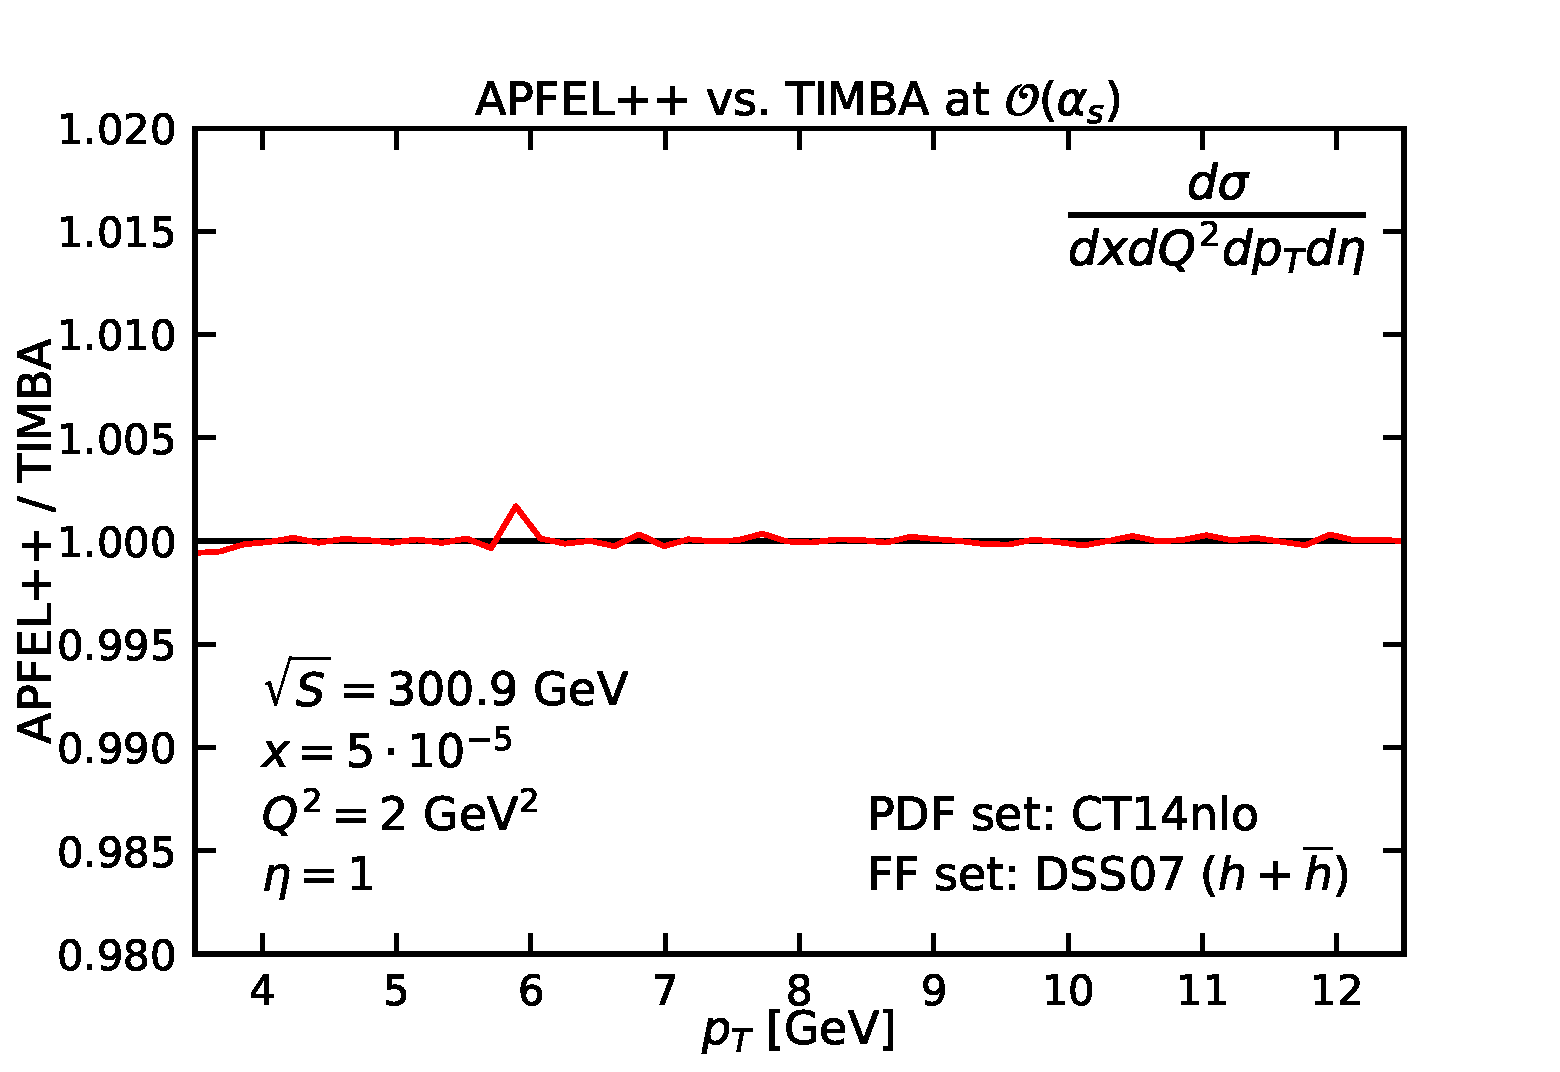
\includegraphics[width=0.6\textwidth]{plots/APFELvsTIMBA}
    \caption{Comparison at $\mathcal{O}(\alpha_s)$ between the {\tt
        TIMBA} code, implementation of the results of
      Ref.~\cite{Daleo:2004pn}, and the implementation of the
      expressions in Eq.~(\ref{eq:FOxsecFin}) in the {\tt APFEL++}
      code~\cite{Bertone:2017gds}.\label{fig:APFELvsTIMBA}}
  \end{centering}
\end{figure}
It is clear that the agreement between the two codes is
excellent. Since we will be using {\tt TIMBA} for the NLO
(\textit{i.e.} $\mathcal{O}(a_s^2)$) cross section calculation to be
matched to the NNLL resummed computation, this provides a solid ground
to start from.

The next step is to compare the asymptotic behaviour worked out in
Eq.~(\ref{eq:FOxsecasy2}) to the fixed-order computation. This is done
Fig.~\ref{fig:FOvsAsy} where the differential cross section in both
cases is plotted as a function of the photon tranverve momentum $q_T$
for a representative set of values of the kinematic variables. As
expected, the two curves are very close to each other at small values
of $q_T$ where the logarithmically enhanced terms dominate. At larger
values of $q_T$ instead the two curves tend to depart indicating that
power corrections are important in that region.
\begin{figure}[t]
  \begin{centering}
    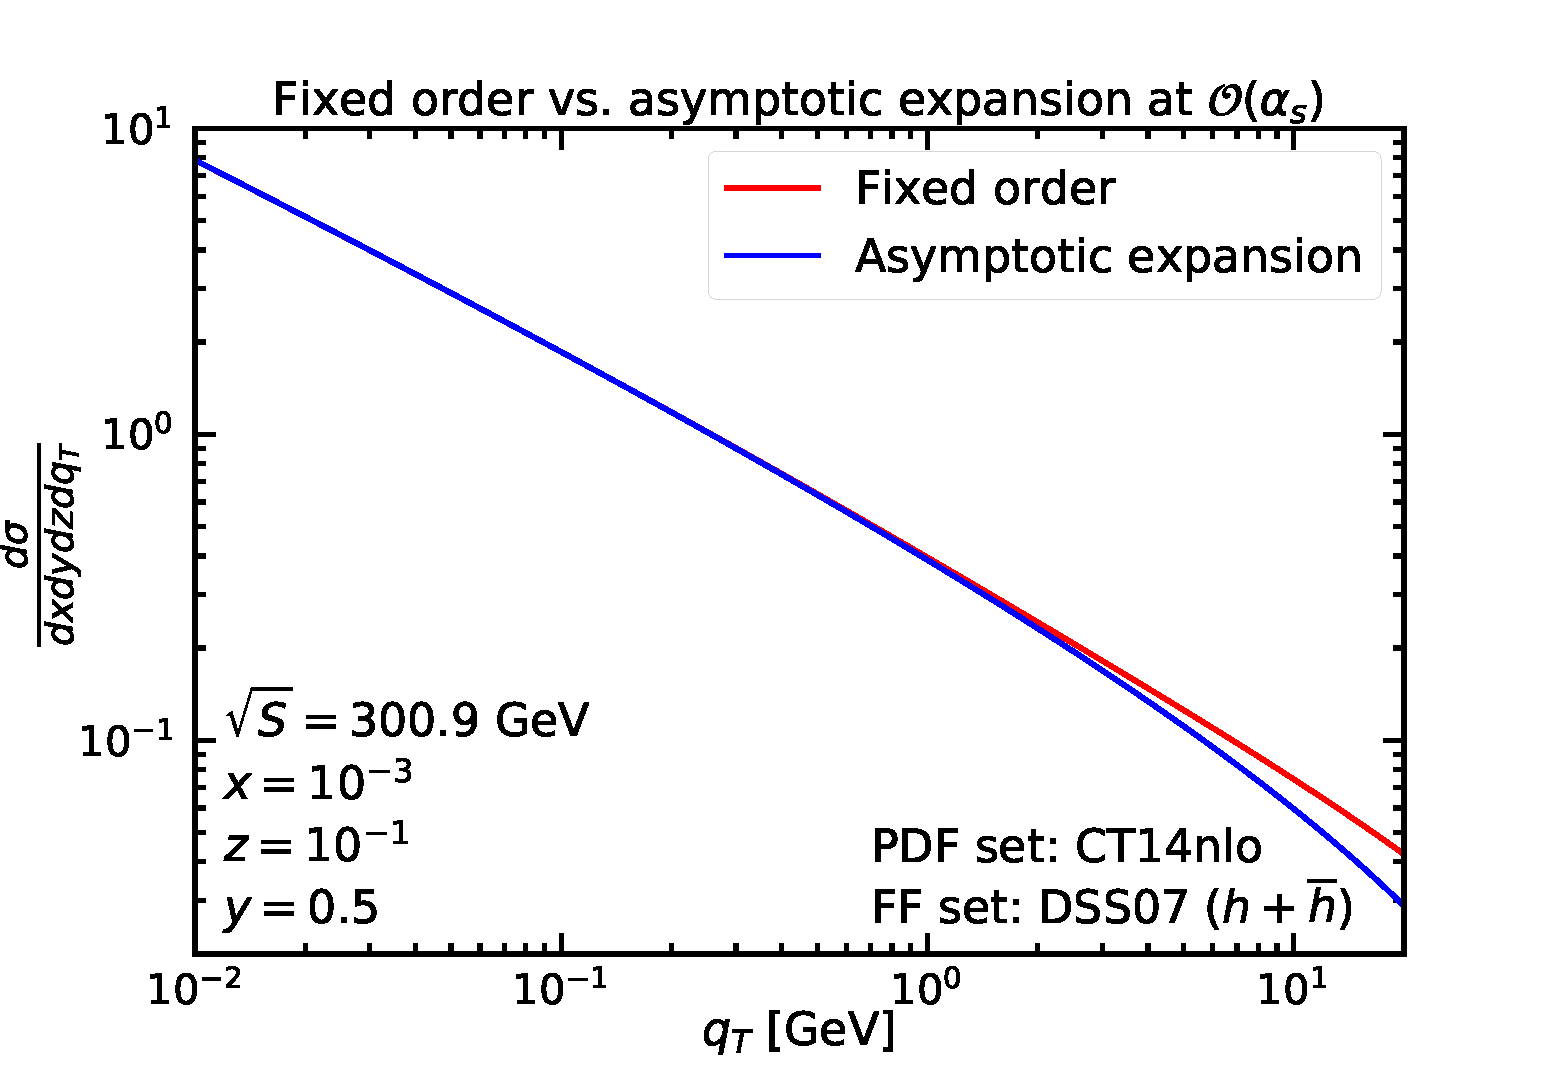
\includegraphics[width=0.6\textwidth]{plots/FOvsAsy}
    \caption{Comparison at $\mathcal{O}(\alpha_s)$ between the
      asymptotic limit in Eq.~(\ref{eq:FOxsecasy2}) to the fixed-order
      computation expressions in
      Eq.~(\ref{eq:FOxsecFin}).\label{fig:FOvsAsy}}
  \end{centering}
\end{figure}

The conclusive step is the comparison between the resummed computation
and its fixed-order order expansion that, as we have shown above,
coincides with the asymptote of the full fixed-oder. This is done in
Fig.~(\ref{fig:ResVsExp}) where the resummed calculation a NLL
accuracy is compared to its fixed-order expansion to
$\mathcal{O}(\alpha_s)$, that coincides with
Eq.~(\ref{eq:FOxsecasy2}). As expected, while the two curves are far
apart at low $q_T$ they tend to converge towards larger values of
$q_T$. However, the convergence is not so ``accurate'' as in the case
of the fixed-order calculation versus its asymptotic limit. The reason
is that in this case the two computations converge up to subleading
terms that in this case are $\mathcal{O}(\alpha_s^2)$ that are
effectively NLO and thus numerically large. We will see that the
situation improves when going one order up.
\begin{figure}[t]
  \begin{centering}
    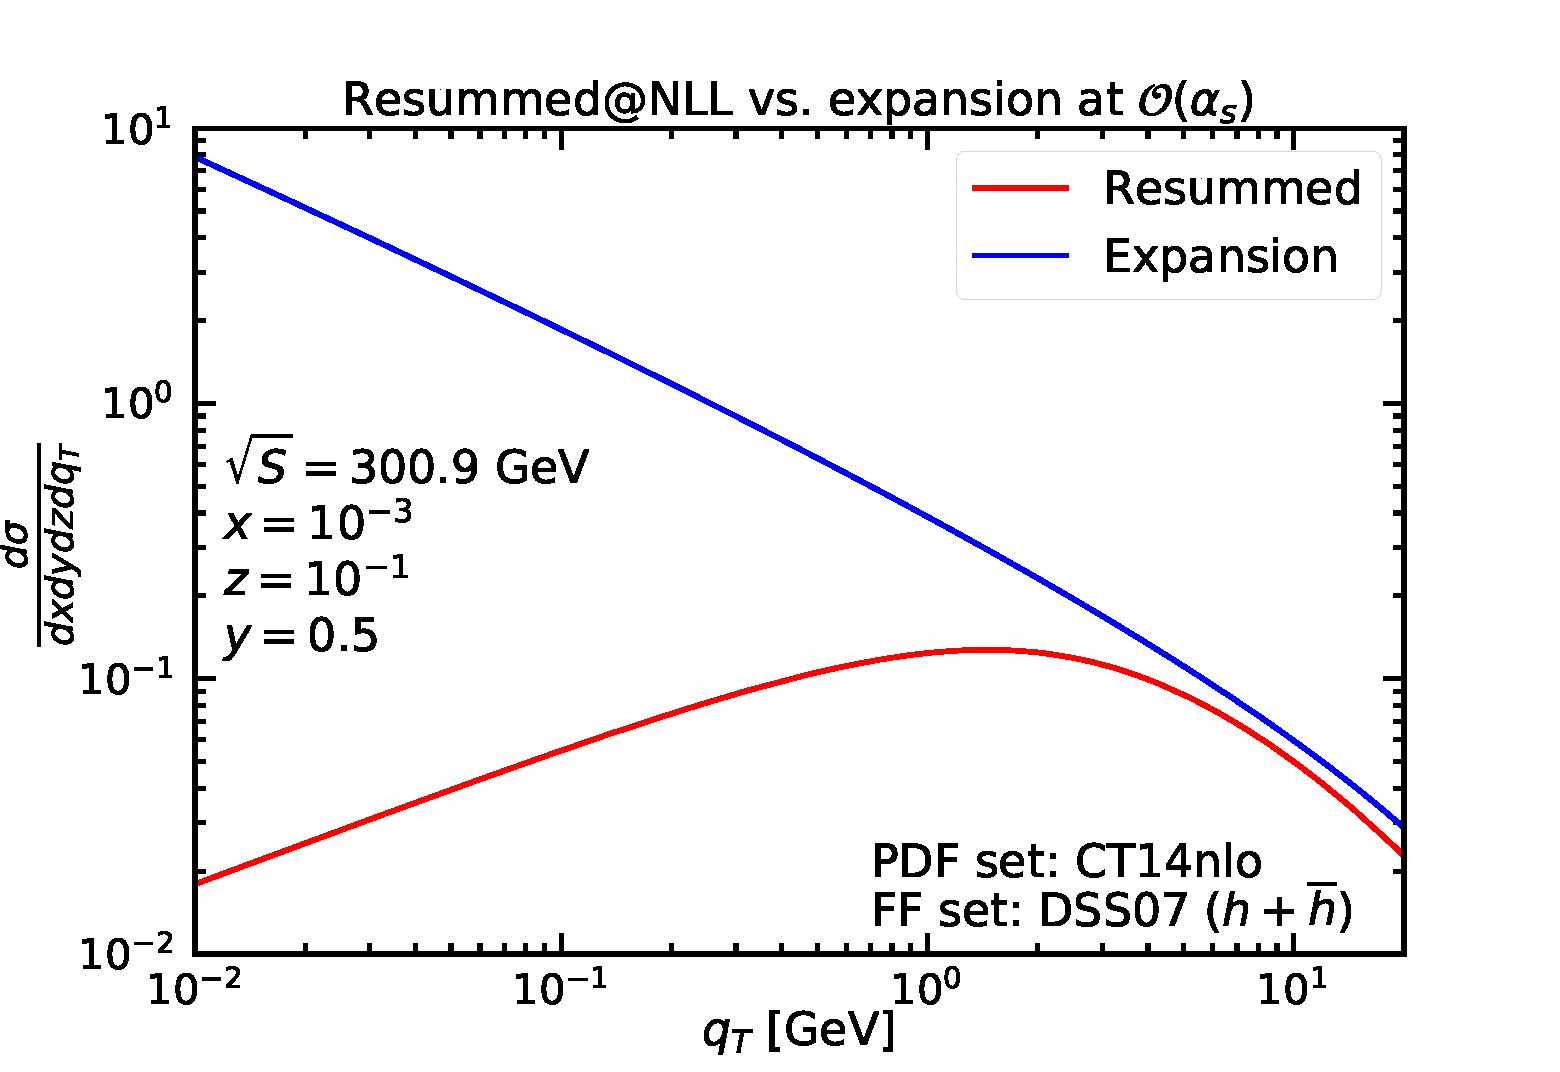
\includegraphics[width=0.6\textwidth]{plots/ResVsExp}
    \caption{Comparison between the NLL resummed calculation and the
      expansion to $\mathcal{O}(\alpha_s)$ in
      Eq.~(\ref{eq:FOxsecasy2}).\label{fig:ResVsExp}}
  \end{centering}
\end{figure}

We can now formulate the matching procedure to consistently combine
the resummed calculation with the fixed-order one subtracting the
double counting terms. The particular way in which the matching is
implemented is defined up to subleading and power-suppressed
terms. One can then exploit this arbitrariness to adjust the matching
in such a way that the possibly large subleading terms are mitigated
by some \textit{ad-hoc} prescription. The most natural, despite not
unique, prescription is the \textit{additive} matching that reads:
\begin{equation}\label{eq:matching1}
\sigma^{\rm Match}(q_T,Q) = \sigma^{\rm FO}(q_T,Q) + \sigma^{\rm Res}(q_T,Q) - \sigma^{\rm Asy}(q_T,Q)\,.
\end{equation}
where $\sigma^{\rm Match}$ is obtained adding up the fixed-order
computation $\sigma^{\rm FO}$ to some perturbative accuracy (say
$\mathcal{O}(\alpha_s^n)$), valid for $q_T \simeq Q$, to the resummed
calculation $\sigma^{\rm Res}$ at some logarithmic accuracy, valid for
$q_T\ll Q$, and subtracting the double-counting terms
$\sigma^{\rm Asy}$. By the arguments discussed above, it is easy to
see that:
\begin{equation}
\begin{array}{rcl}
  \sigma^{\rm Match}(q_T,Q) &\displaystyle\mathop{\longrightarrow}_{q_T\simeq Q}&
                                                                                  \sigma^{\rm FO}(q_T,Q) +\mathcal{O}\left[\alpha_s^{n+1}(Q)\right]\,,\\
  \\
  \sigma^{\rm Match}(q_T,Q) &\displaystyle\mathop{\longrightarrow}_{q_T\ll Q}&\displaystyle
                                                                               \sigma^{\rm Res}(q_T,Q) +\mathcal{O}\left(\frac{q_T^2}{Q^2}\right)\,.
\end{array}
\end{equation}
However, as we have seen above, for low-order computation the
$\mathcal{O}(\alpha_s^{n+1})$ residual for $q_T\simeq Q$ may be
numerically relevant.

% Exploiting the power-suppressed residual in the $q_T \ll Q$ limit, one
% can replace the prescription in Eq.~(\ref{eq:matching1}) with:
% \begin{equation}\label{eq:matching2}
%   \sigma^{\rm Match}(q_T,Q) = \sigma^{\rm FO}(q_T,Q) + \mathcal{D}\left(\frac{q_T^2}{Q^2}\right)\left[\sigma^{\rm Res}(q_T,Q) - \sigma^{\rm Asy}(q_T,Q)]\right]\,,
% \end{equation}
% with:
% \begin{equation}
% \mathcal{D}\left(\frac{q_T^2}{Q^2}\right) = 1 + \mathcal{O}\left(\frac{q_T^2}{Q^2}\right)\,.
% \end{equation}
% Despite the exact form of the ``damping'' function $\mathcal{D}$
% remains unspecified at this level, this prescription ensures that the
% uncertainty of Eq.~(\ref{eq:matching2}) is power suppressed over the
% whole relevant spectrum. The simplest choice is:
% \begin{equation}
%   \mathcal{D}\left(\frac{q_T^2}{Q^2}\right) = 1 + \frac{q_T^2}{Q^2}\,.
% \end{equation}



\newpage

\begin{thebibliography}{alp}

%\cite{Scimemi:2017etj}
\bibitem{Scimemi:2017etj}
  I.~Scimemi and A.~Vladimirov,
  %``Analysis of vector boson production within TMD factorization,''
  arXiv:1706.01473 [hep-ph].
  %%CITATION = ARXIV:1706.01473;%%
  %2 citations counted in INSPIRE as of 24 Oct 2017

%\cite{Echevarria:2016scs}
\bibitem{Echevarria:2016scs}
  M.~G.~Echevarria, I.~Scimemi and A.~Vladimirov,
  %``Unpolarized Transverse Momentum Dependent Parton Distribution and Fragmentation Functions at next-to-next-to-leading order,''
  JHEP {\bf 1609} (2016) 004
  doi:10.1007/JHEP09(2016)004
  [arXiv:1604.07869 [hep-ph]].
  %%CITATION = doi:10.1007/JHEP09(2016)004;%%
  %20 citations counted in INSPIRE as of 19 Dec 2017

%\cite{vanNeerven:2000uj}
\bibitem{vanNeerven:2000uj}
  W.~L.~van Neerven and A.~Vogt,
  %``NNLO evolution of deep inelastic structure functions: The Singlet case,''
  Nucl.\ Phys.\ B {\bf 588} (2000) 345
  doi:10.1016/S0550-3213(00)00480-6
  [hep-ph/0006154].
  %%CITATION = doi:10.1016/S0550-3213(00)00480-6;%%
  %159 citations counted in INSPIRE as of 19 Dec 2017

%\cite{Bozzi:2005wk}
\bibitem{Bozzi:2005wk}
  G.~Bozzi, S.~Catani, D.~de Florian and M.~Grazzini,
  %``Transverse-momentum resummation and the spectrum of the Higgs boson at the LHC,''
  Nucl.\ Phys.\ B {\bf 737} (2006) 73
  doi:10.1016/j.nuclphysb.2005.12.022
  [hep-ph/0508068].
  %%CITATION = doi:10.1016/j.nuclphysb.2005.12.022;%%
  %362 citations counted in INSPIRE as of 20 Dec 2017

%\cite{Meng:1995yn}
\bibitem{Meng:1995yn}
  R.~Meng, F.~I.~Olness and D.~E.~Soper,
  %``Semiinclusive deeply inelastic scattering at small q(T),''
  Phys.\ Rev.\ D {\bf 54} (1996) 1919
  doi:10.1103/PhysRevD.54.1919
  [hep-ph/9511311].
  %%CITATION = doi:10.1103/PhysRevD.54.1919;%%
  %49 citations counted in INSPIRE as of 21 Dec 2017

%\cite{Collins:2016hqq}
\bibitem{Collins:2016hqq}
  J.~Collins, L.~Gamberg, A.~Prokudin, T.~C.~Rogers, N.~Sato and B.~Wang,
  %``Relating Transverse Momentum Dependent and Collinear Factorization Theorems in a Generalized Formalism,''
  Phys.\ Rev.\ D {\bf 94} (2016) no.3,  034014
  doi:10.1103/PhysRevD.94.034014
  [arXiv:1605.00671 [hep-ph]].
  %%CITATION = doi:10.1103/PhysRevD.94.034014;%%
  %14 citations counted in INSPIRE as of 21 Dec 2017

%\cite{Nadolsky:1999kb}
\bibitem{Nadolsky:1999kb}
  P.~M.~Nadolsky, D.~R.~Stump and C.~P.~Yuan,
  %``Semiinclusive hadron production at HERA: The Effect of QCD gluon resummation,''
  Phys.\ Rev.\ D {\bf 61} (2000) 014003
   Erratum: [Phys.\ Rev.\ D {\bf 64} (2001) 059903]
  doi:10.1103/PhysRevD.64.059903, 10.1103/PhysRevD.61.014003
  [hep-ph/9906280].
  %%CITATION = doi:10.1103/PhysRevD.64.059903, 10.1103/PhysRevD.61.014003;%%
  %77 citations counted in INSPIRE as of 23 Dec 2017

%\cite{Bacchetta:2008xw}
\bibitem{Bacchetta:2008xw}
  A.~Bacchetta, D.~Boer, M.~Diehl and P.~J.~Mulders,
  %``Matches and mismatches in the descriptions of semi-inclusive processes at low and high transverse momentum,''
  JHEP {\bf 0808} (2008) 023
  doi:10.1088/1126-6708/2008/08/023
  [arXiv:0803.0227 [hep-ph]].
  %%CITATION = doi:10.1088/1126-6708/2008/08/023;%%
  %174 citations counted in INSPIRE as of 25 Dec 2017

%\cite{Daleo:2004pn}
\bibitem{Daleo:2004pn}
  A.~Daleo, D.~de Florian and R.~Sassot,
  %``O(alpha**2(s)) QCD corrections to the electroproduction of hadrons with high transverse momentum,''
  Phys.\ Rev.\ D {\bf 71} (2005) 034013
  doi:10.1103/PhysRevD.71.034013
  [hep-ph/0411212].
  %%CITATION = doi:10.1103/PhysRevD.71.034013;%%
  %45 citations counted in INSPIRE as of 25 Dec 2017

%\cite{Bertone:2017gds}
\bibitem{Bertone:2017gds}
  V.~Bertone,
  %``APFEL++: A new PDF evolution library in C++,''
  arXiv:1708.00911 [hep-ph].
  %%CITATION = ARXIV:1708.00911;%%
  %3 citations counted in INSPIRE as of 30 Dec 2017

\end{thebibliography}

\end{document}
